\section{Day 1: Hall's Theorem (Jan. 8, 2025)}
The course textbook is Van Lint and Wilson, link \href{https://mathematicalolympiads.wordpress.com/wp-content/uploads/2012/08/a_course_in_combinatorics.pdf}{here}. The grading scheme is given by
\begin{enumerate}[label=(\roman*)]
    \item 30\% Scribing: i.e., writing out the lecture notes on LaTeX;
    \item 30\% Homeworks;
    \item 40\% Final Exam.
\end{enumerate}
The knowledge prerequisites for this class are linear algebra, basic discrete probability, and simple combinatorics. This class is about combinatorial and discrete objects, and extremal problems about them.
\medskip\newline
As an example, consider $[n] = \{1, \dots, n\}$, and $\alpha \geq \beta \in [0, 1]$. We want $A_1, \dots A_k \subseteq [n]$ such that $\abs{A_i} \geq \alpha n$ for all $i$, with $\abs{A_i \cap A_j} \leq \beta n$. How big can $k$ be? What are the asymptotics as $n \to \infty$ if we leave $\alpha, \beta$ fixed? Consider the following square,
\begin{figure}[h] \centering 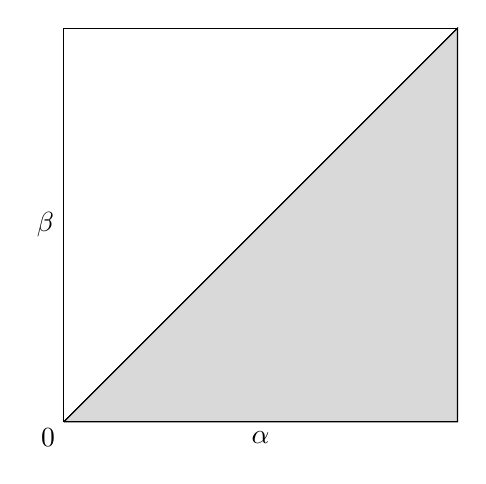
\begin{tikzpicture}
    \draw[fill=gray!30] (0, 0) -- (5, 0) -- (5, 5) -- (0, 0);
    \draw (0, 0) -- node[below]{$\alpha$}(5, 0) -- (5, 5) -- (0, 5) -- node[left]{$\beta$}(0, 0);
    \node at (-0.2, -0.2) {$0$}; %fuck it
    \draw (0, 0) -- (5, 5);
\end{tikzpicture} \end{figure}
where the gray triangle represents the possible choices of $\alpha, \beta$.\footnote{additional details on example choices of $\alpha, \beta$ omitted because i'm garbage at using tikz} We may note that
\[ k \geq \binom{n}{\frac{n}{2}} \approx O\left( \frac{2^n}{\sqrt{n}} \right). \]
We now work to introduce Hall's Theorem. Consider a bipartite graph, with $n$ vertices on both sides (where we will let $V = L \sqcup R$), and the edge set $E \subseteq L \times R$.
\begin{definition}
    A \textit{perfect matching} on $V$ is a matching wtih $n$ edges.
\end{definition}
\noindent With this in mind, we ask; when does a bipartite graph have a perfect matching? To start, if a graph does not admit a perfect matching, then there exists a subset of $L$ in which the number of neighbors is less than the number of elements in the set. Formally writing, if $G$ has a perfect matching, then for all subsets $S \subseteq L$, $\abs{N(S)} \geq \abs{S}$ (where $N(S)$ represents the set of neighbors of $S$). Similarly, its contrapositive states that if there exists some $S \subseteq L$ such that $\abs{N(S)} < \abs{S}$, then there does not exist a perfect matching.
\begin{simplethm}[Hall's Theorem]
    If $G$ does not have a perfect matching, then there exists $S \subseteq L$ such that $\abs{N(S)} \leq \abs{S}$.
\end{simplethm}
\noindent We start with an inductive proof on $n$. Start with a graph $G$ such that for all $S \subseteq L$, $\abs{N(S)} \geq \abs{S}$; we want to find a perfect matching for $G$. Proceed with casework;
\begin{itemize}
    \item In the first case (in which there is slack), suppose that for all nonempty, non-whole subsets $S \subseteq L$, $\abs{N(S)} \geq \abs{S}$. Take any edge $e = (x, y) \in E$, and delete it to get $G' = (L \setminus \{x\}, R \setminus \{y\}, E')$, where $E' = E \setminus \{e\}$. Then $G'$ satisfies the inductive hypothesis, without slack.
    \item In the second case (in which there is no slack), there exists $S \subseteq L$ such that $S \neq \emptyset, L$ such that $\abs{N(S)} = \abs{S}$. Produce graph $G' = (S, N(S), E \cap (S \times N(S)))$. $G'$ satisfies the inductive hypothesis, since its neighborhoods are the same as in $G$. For $T \subseteq S$, $N_{G'}(T) = N_G(T)$, so $G'$ indeed has a perfect matching $M'$.
    \medskip\newline
    Now, produce another graph $G'' = (L \setminus S, R \setminus N(S), E \cap (L \setminus S) \times (R \setminus N(S)))$; we want to show that $G''$ satisfies Hall's condition. Take $T \subseteq L \setminus S$; we have that $\abs{N_G(T)} \geq \abs{T}$. Consider $T \cup S$; $N_G(T \cup S) = N_G(S) \sqcup N_{G''}(T)$ and $\abs{N_G(S)} = \abs{S}$, so $\abs{N_{G''}(T)} \geq \abs{T}$. Thus, we conclude that $G''$ satisfies Hall's conditoion, and so it has a perfect matching $M''$. Then we may take $M = M' \cup M''$ as our desired perfect matching for $G$. \qed
\end{itemize}
Here are a handful of trivial algorithms to determine perfect matching;
\begin{enumerate}[label=(\alph*)]
    \item If we check all subsets of $E$, then it would take $2^{O(n^2)}$ time.
    \item All bijections between $L, R$, and check if the subsets of $E$ work; this would take $O(n!) \leq n^n = 2^{O(n \log n)}$.
    \item Hall's condition takes $O(n^2 \cdot 2^n)$ time.\footnote{not sure what this means...}
\end{enumerate}
We now present an algebraic algorithm for checking if a bipartite graph has a perect matching. Consider the $n \times n$ adjacency matrix $A_G$ between $L$ and $R$, where an entry is $1$ if $(x, y)$ is an edge (with $x \in L, y \in R$), and $0$ otherwise. Now, replace each $1$ in $A_G$ with a random value in $[0, 1]$, and call the new matrix $B_G$. Compute $\det B_G$. If $\det B_G = 0$, then there is no perfect matching; otherwise, there is a perfect matching with probability $1$.
\medskip\newline
Consider the variable adjacency matrix $M_G((x_e)_{e \in E})$, where $P(\vec{x}) = \det M_G(\vec{x})$, with $\vec{x} \in [0, 1]^E$. Compute $P(\vec{x})$. For example, if
\[ M_G = \begin{pmatrix} x_1 & 0 \\ x_2 & 0 \end{pmatrix}, \]
then $P(\vec{x}) = 0$. However, if
\[ M_G = \begin{pmatrix} x_1 & x_2 \\ x_3 & x_4 \end{pmatrix}, \]
then $P(\vec{x}) = \det M_G = x_1 x_4 - x_2 x_3$. It is extremely unlikely that $P(\vec{x}) = 0$, and so we have our algorithm as desired.
\begin{simplelemma}
    $G$ has a perfect matching if and only if $p(\vec{x}) \neq 0$.
\end{simplelemma}
\begin{simplelemma}
    If $Q(x_1, \dots, x_m)$ is a nonzero polynomial, then
    \[ \mathrm{Pr}_{x \in [0, 1]^m} [Q(x) = 0] = 0. \]
\end{simplelemma}
\begin{simplelemma}[\href{https://en.wikipedia.org/wiki/Schwartz\%E2\%80\%93Zippel_lemma}{Schwartz-Zippel}]
    Let $S \subseteq \FF$. If $Q(x_1, \dots, x_m) \in \FF[x_1, \dots, x_m]$ is nonzero of degree $\leq d$, then
    \[ \mathrm{Pr}_{x \in S^m}[Q(x) = 0] \leq \frac{d}{\abs{S}}. \]
\end{simplelemma}
\noindent We will now prove this. To start,
\[ P(\vec{x}) = \det M_Q(\vec{x}) = \sum_{\pi : L \to R} (-1)^{\mathrm{sgn}(\pi)} \prod_{u \in L} M_{(u, \pi(u))}, \]
which is an equivalent expression to
\[ \sum_{\substack{\text{perf. matchings} \\ \pi : L \to R }} \pm \prod_{u \in L} X_{(u, \pi(u))}. \]
The \textit{permanent} here is essentially the number of perfect matchings. In general, determinants are easy to compute, but permanents are hard.
\medskip\newline
We now prove the Schwartz-Zippel lemma. Let $Q(x_1, \dots, x_m)$ be nonzero with degree $\leq d$. We claim that the number of $a = (a_1, \dots, a_n) \in S^n$ such that $Q(a) = 0$ is less than or equal to $d \abs{S}^{n-1}$. Proceed by casework;
\begin{itemize}
    \item For $m = 1$, by the fundamental theorem of algebra, an nonzero univariate polynomial of degree $d$ has at most $d$ roots.
    \item We now induct on $m$. Write
    \[ Q(x_1, \dots, x_m) = x^t_m Q_t(x_1, \dots, x_{m-1}) + \dots + Q_0(x_1, \dots, x_{m-1}) \]
    as a polynomial in $x_m$. Note that $\deg Q_i \leq d - i$, and that $Q_t \neq 0$. Let $B = \{ (a_1, \dots, a_{m-1}) \in S^{n-1} \mid Q_t(a_1, \dots, a_{m-1}) = 0 \}$. Then by the induction hypothesis, we have
    \[ \mathrm{Pr}_{(a_1, \dots, a_{n-1}) \in S^{n-1}} [(a_1, \dots, a_{m-1}) \in B] \leq \frac{\deg Q_i}{\abs{S}} \leq \frac{d - t}{\abs{S}}. \]
    If $(a_1, \dots, a_{m-1}) \not\in B$, then
    \[ \mathrm{Pr}_{a_m \in S} [Q(a_1, \dots, a_m) = 0] \leq \frac{t}{\abs{S}}. \]
    I don't entirely understand where this is going because it's notation hell, but I know the proof I guess. Read wikipedia \href{https://en.wikipedia.org/wiki/Schwartz%E2%80%93Zippel_lemma}{link :p} hehe.
\end{itemize}
\begin{definition}[Doubly-Stochastic Matrix]
    A doubly stochastic matrix is $M \in \RR^{n \times n}$ such that $M_{ij} \geq 0$ for all $i, j$, and for all $i$, $\sum_j M_{ij} = 1$, and for all $j$, $\sum_i M_{ij} = 1$; i.e., the rows and columns sum to $1$.
\end{definition}
\noindent Every doubly stochastic matrix is a convex combination of permutation matrices. (Birkhoff's Theorem, \href{https://webpages.charlotte.edu/ghetyei/courses/old/F13.3116/birkhofft.pdf}{here}, and Theorem 5.5 in textbook)
\medskip\newline
Leaving off notes for today because I need to go find where MAT267 is.